% Generated by code/scripts/report_figures.py at 2026-11-07T04:44:01Z; do not edit.
% Inputs: artifacts/cluster/runs/bench1-20261107T033925Z-1528774
\begin{figure}[t]
\centering
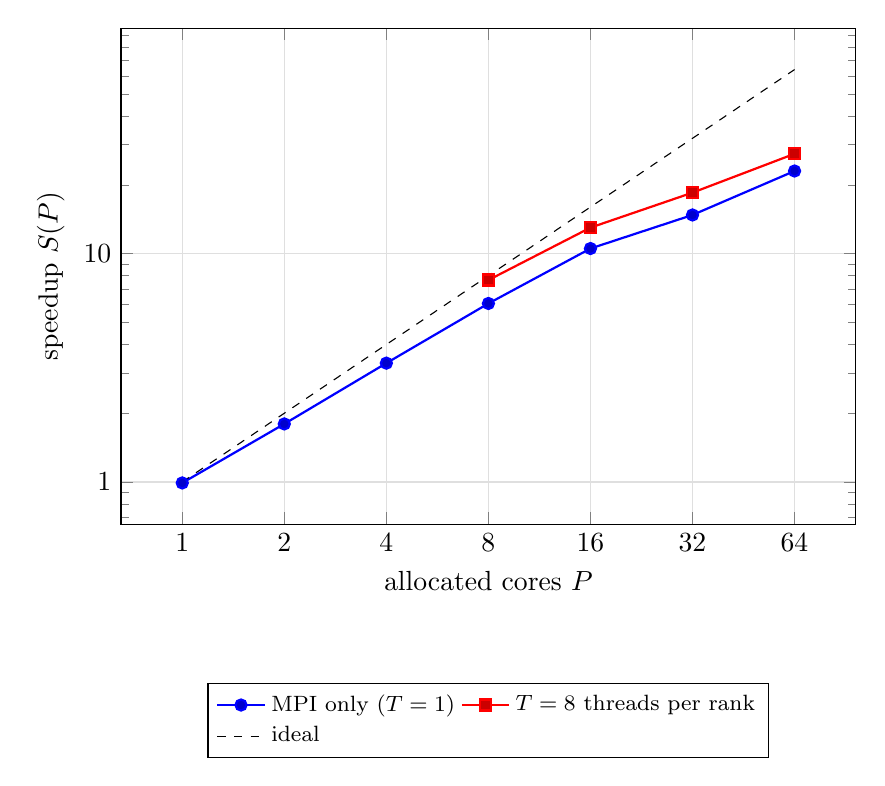
\begin{tikzpicture}
\begin{axis}[width=0.9\columnwidth, height=0.65\columnwidth, xlabel={allocated cores $P$}, ylabel={speedup $S(P)$}, xmode=log, log basis x=2, log ticks with fixed point, ymode=log, ytick={0.1,1,10,100}, legend style={at={(0.5,-0.32)}, anchor=north, legend columns=2, font=\footnotesize}, legend cell align=left, grid=major, grid style={gray!25}]
\addplot+[mark=*, thick] coordinates {(1,0.9905) (2,1.796) (4,3.315) (8,6.05) (16,10.53) (32,14.77) (64,23.01)};
\addlegendentry{MPI only ($T=1$)}
\addplot+[mark=square*, thick] coordinates {(8,7.663) (16,13) (32,18.5) (64,27.37)};
\addlegendentry{$T=8$ threads per rank}
\addplot[black, dashed] coordinates {(1,1) (64,64)};
\addlegendentry{ideal}
\end{axis}
\end{tikzpicture}
\caption{Strong-scaling speedup. $N=1000000$, median of repetitions; serial Barnes--Hut baseline on the same CPU model and build. Vanda job 1528774: all 64 cores of Gold 6438N node IN-008, 3 interleaved repetitions.}
\label{fig:strong-speedup}
\end{figure}
